\documentclass[12pt, titlepage]{article}

\usepackage{fullpage}
\usepackage[round]{natbib}
\usepackage{multirow}
\usepackage{booktabs}
\usepackage{tabularx}
\usepackage{graphicx}
\usepackage{float}
\usepackage{hyperref}
\usepackage{xcolor}
\usepackage{soul}
\hypersetup{
	colorlinks,
	citecolor=black,
	filecolor=black,
	linkcolor=red,
	urlcolor=blue
}
\usepackage[round]{natbib}

\newcounter{acnum}
\newcommand{\actheacnum}{AC\theacnum}
\newcommand{\acref}[1]{AC\ref{#1}}

\newcounter{ucnum}
\newcommand{\uctheucnum}{UC\theucnum}
\newcommand{\uref}[1]{UC\ref{#1}}

\newcounter{mnum}
\newcommand{\mthemnum}{M\themnum}
\newcommand{\mref}[1]{M\ref{#1}}

\title{SE 3XA3: Module Guide\\ Wordle 2.0}

\author{Team 8,
	\\ Richard Fan, fanr13
	\\ Noel Zacharia, zacharin
	\\ Biranugan Pirabaharan, pirabahb
}

\date{\today}

\begin{document}
	
	\maketitle
	
	\pagenumbering{roman}
	\tableofcontents
	\listoftables
	\listoffigures
	
	\begin{table}[bp]
		\caption{\bf Revision History}
		\begin{tabularx}{\textwidth}{p{3cm}p{2cm}X}
			\toprule {\bf Date} & {\bf Version} & {\bf Notes}\\
			\midrule
			March 12, 2022 & 0.1 & Initial document\\
			March 18, 2022 & 0.2 & Finished MG\\
			April 10, 2022 & 0.3 & Updated for Rev1\\
			\bottomrule
		\end{tabularx}
	\end{table}
	
	\newpage
	
	\pagenumbering{arabic}
	
	\section{Introduction}
	\subsection{Overview}
	Wordle 2.0 is a re-implementation of the game Not Wordle. The original game made players guess a 5 letter word in 6 tries. The purpose of this project is to recreate the functionality of the original game while also adding additional features to create extra value. Additionally, we have followed the software development process to ensure that our system is well built and understood by others. 
	\subsection{Purpose}
	The Module Guide serves as a guide to the modular structure of our system. The system is decomposed into several modules based on the design principle of information hiding~\citep{Parnas1972a}. This method allows maintainers, new project members, and designers to quickly understand different parts of the system, allowing for high maintainability and readability. Additionally, this design principle also supports the idea of design for change and information hiding since likely changes can be hidden as "secrets" within individual modules.
	\subsection{Scope}
	This Module Guide describes the modules that are based upon the requirements found within the Software Requirements Specification. External behaviors of these modules will be described in the Module Interface Specification (MIS) document. Likely and unlikely changes are documented. A use hierarchy is provided to visualize use relations between modules specified in this document.
	\subsection{Outline}
	The rest of the document is structured as follows:
	
	\begin{itemize}
		\item Section \ref{SecChange} lists the anticipated and unlikely changes of the software requirements. 
		\item Section \ref{SecMH} summarizes the module decomposition that was constructed according to the likely changes. 
		\item Section \ref{SecConnection} specifies the connections between the software requirements and the modules. \item Section \ref{SecMD} gives a detailed description of the modules. 
		\item Section \ref{SecTM} includes two traceability matrices. One checks the completeness of the design against the requirements provided in the SRS. The other shows the relation between anticipated changes and the modules. 
		\item Section \ref{SecUse} describes the use relation between modules. 
	\end{itemize}
	
	
	
	
	
	\section{Anticipated and Unlikely Changes} \label{SecChange}
	
	This section lists possible changes to the system. According to the likeliness
	of the change, the possible changes are classified into two
	categories. Anticipated changes are listed in Section \ref{SecAchange}, and
	unlikely changes are listed in Section \ref{SecUchange}.
	
	\subsection{Anticipated Changes} \label{SecAchange}
	
	Anticipated changes are the source of the information that is to be hidden
	inside the modules. Ideally, changing one of the anticipated changes will only
	require changing the one module that hides the associated decision. The approach
	adapted here is called design for
	change.
	
	\begin{description}
		\item[\refstepcounter{acnum} \actheacnum \label{ac1}:] The graphical elements used in the game will be improved and revised over time. The web page will feature a more polished appearance for the final deliverable. 
		\item[\refstepcounter{acnum} \actheacnum \label{ac2}:] The theme options the player has to choose from will have options and be refined. The current dark mode will be completely reworked as its current implementation was just a placeholder. 
		\item[\refstepcounter{acnum} \actheacnum \label{ac3}:] The algorithm used to find the accuracy of the guesses. Currently, any occurrences of letters that are present in the target word are shown as present even when the target word has fewer occurrences than the guess itself. 
		\item[\refstepcounter{acnum} \actheacnum \label{ac4}:] The appearance of the game's alert system for invalid guesses and guesses that are too short. Currently uses the browser's default alert.
		\item[\refstepcounter{acnum} \actheacnum \label{ac5}:] Additional functionality that has yet to be added: various word lengths support. 
		
	\end{description}
	
	\subsection{Unlikely Changes} \label{SecUchange}
	
	The module design should be as general as possible. However, a general system is
	more complex. Sometimes this complexity is not necessary. Fixing some design
	decisions at the system architecture stage can simplify the software design. If
	these decision should later need to be changed, then many parts of the design
	will potentially need to be modified. Hence, it is not intended that these
	decisions will be changed.
	
	\begin{description}
		\item[\refstepcounter{ucnum} \uctheucnum] Input methods of the user
		(Input: mouse and/or keyboard). 
		\item[\refstepcounter{ucnum} \uctheucnum] The word lists used for determining the target word and accepting the guesses. These are static lists with over 2000 possible words.
		\item[\refstepcounter{ucnum} \uctheucnum] The keyboard and its layout. The game will not support unconventional layouts. It will stick to QWERTY. Additionally, only modern English letters will be supported, with no accents or other language options. 
		\item[\refstepcounter{ucnum} \uctheucnum] The core rules of the game.
	\end{description}
	
	\section{Module Hierarchy} \label{SecMH}
	
	This section provides an overview of the module design. Modules are summarized
	in a hierarchy decomposed by secrets in Table \ref{TblMH}. The modules listed
	below, which are leaves in the hierarchy tree, are the modules that will
	actually be implemented.
	
	\begin{description}
		\item [\refstepcounter{mnum} \mthemnum \label{m1}:]
		Valid Guess
		\item [\refstepcounter{mnum} \mthemnum \label{m2}:]
		Word Operations
		\item [\refstepcounter{mnum} \mthemnum \label{m3}:]
		Create Gameboard
		\item [\refstepcounter{mnum} \mthemnum \label{m4}:]
		Dark Mode
		\item [\refstepcounter{mnum} \mthemnum \label{m5}:]
		Main
		\item [\refstepcounter{mnum} \mthemnum \label{m6}:]
		Keyboard Colours
		\item [\refstepcounter{mnum} \mthemnum \label{m7}:]
		Tile Colours
		\item [\refstepcounter{mnum} \mthemnum
		\label{m8}:]
		\st{Keyboard}
		\item [\refstepcounter{mnum} \mthemnum
		\label{m9}:]
		Stats
		\item [\refstepcounter{mnum} \mthemnum
		\label{m10}:]
		Instructions
		\item [\refstepcounter{mnum} \mthemnum
		\label{m11}:]
		Stats View
		\item [\refstepcounter{mnum} \mthemnum
		\label{m12}:]
		Constants
		\item [\refstepcounter{mnum} \mthemnum
		\label{m13}:]
		Update Gameboard
		\item [\refstepcounter{mnum} \mthemnum
		\label{m14}:]
		Style
		\item [\refstepcounter{mnum} \mthemnum \label{m15}:]
		Alert
		\item [\refstepcounter{mnum} \mthemnum
		\label{m16}:]
		Click
		\item [\refstepcounter{mnum} \mthemnum
		\label{m17}:]
		Index
		\item [\refstepcounter{mnum} \mthemnum
		\label{m18}:]
		Share
		
		
		
	\end{description}
	
	
	\begin{table}[h!]
		\centering
		\begin{tabular}{p{0.3\textwidth} p{0.6\textwidth}}
			\toprule
			\textbf{Level 1} & \textbf{Level 2}\\
			\midrule
			
			{Hardware-Hiding Module} & ~ \\
			\midrule
			
			\multirow{7}{0.3\textwidth}{Behaviour-Hiding Module} & Stats View \\
			& \st{Keyboard}\\
			& Dark Mode\\
			& Instructions\\
			& Keyboard Colours\\
			& Tile Colours\\
			& Create Gameboard\\ 
			& Style\\
			& Alert\\
			& Click\\
			& Index\\
			& Share\\
			& Update Gameboard\\
			\midrule
			
			\multirow{3}{0.3\textwidth}{Software Decision Module} & {Word Operations}\\
			& Stats\\
			& Valid Guess\\
			& Main\\
			& Constants\\
			\bottomrule
			
		\end{tabular}
		\caption{Module Hierarchy}
		\label{TblMH}
	\end{table}
	
	\section{Connection Between Requirements and Design} \label{SecConnection}
	The system encompassing Wordle 2.0 is designed to satisfy all of the functional and non-functional requirements that were laid out in the SRS. The system is decomposed into modules and the connections between the requirements and modules are shown via traceability matrices in Table \ref{TblRT}.
	
	Modules are decomposed such that every requirement we outlined can be traced to at least one module. The module name is indicative of the module functioning.
	
	\section{Module Decomposition} \label{SecMD}
	
	Modules are decomposed according to the principle of ``information hiding''
	proposed by \citet{ParnasEtAl1984}. The \emph{Secrets} field in a module
	decomposition is a brief statement of the design decision hidden by the
	module. The \emph{Services} field specifies \emph{what} the module will do
	without documenting \emph{how} to do it. For each module, a suggestion for the
	implementing software is given under the \emph{Implemented By} title. If the
	entry is \emph{OS}, this means that the module is provided by the operating
	system or by standard programming language libraries.  Also indicate if the
	module will be implemented specifically for the software.
	
	Only the leaf modules in the
	hierarchy have to be implemented. If a dash (\emph{--}) is shown, this means
	that the module is not a leaf and will not have to be implemented. Whether or
	not this module is implemented depends on the programming language
	selected.
	
	\subsection{Hardware Hiding Modules}
	N/A
	
	\subsection{Behaviour Hiding Modules}
	
	\subsubsection{Create Gameboard (\mref{m3})}
	
	\begin{description}
		\item[Secrets:]The method of drawing the gameboard to the screen.
		\item[Services:]Draws the gameboard to the screen.
		\item[Implemented By:] Wordle 2.0
	\end{description}
	
	\subsubsection{Dark Mode (\mref{m4})}
	\begin{description}
		\item[Secrets:]The method of changing the background to dark mode.
		\item[Services:]Changes the the background to dark mode.
		\item[Implemented By:] Wordle 2.0
	\end{description}
	
	\subsubsection{Keyboard Colours (\mref{m6})}
	\begin{description}
		\item[Secrets:]The method for changing key colours to green, yellow, and grey.
		\item[Services:]Changes key colours.
		\item[Implemented By:] Wordle 2.0
	\end{description}
	
	\subsubsection{Tile Colours (\mref{m7})}
	\begin{description}
		\item[Secrets:]The method for changing gameboard tile colours to green, yellow, and grey.
		\item[Services:]Changes tile colours within the gameboard.
		\item[Implemented By:] Wordle 2.0
	\end{description}
	
	\subsubsection{Keyboard (\mref{m8})}
	\begin{description}
		\item[Secrets:]\st{The method for drawing the keyboard to the screen.}
		\item[Services:]\st{Draws the keyboard to the screen.}
		\item[Implemented By:] \st{Wordle 2.0}
	\end{description}
	
	\subsubsection{Instructions (\mref{m10})}
	\begin{description}
		\item[Secrets:]The method to visualize the instructions screen.
		\item[Services:]Draws the instructions menu with a GUI.
		\item[Implemented By:] Wordle 2.0
	\end{description}
	
	\subsubsection{Stats View (\mref{m11})}
	\begin{description}
		\item[Secrets:]The method to visualize the statistics screen.
		\item[Services:]Draws the statistics menu with a GUI.
		\item[Implemented By:] Wordle 2.0
	\end{description}
	
	\subsubsection{Update Gameboard (\mref{m13})}
	\begin{description}
		\item[Secrets:]The method to update the gameboard with the provided letter.
		\item[Services:] Updates the gameboard with the provided letter
		\item[Implemented By:] Wordle 2.0
	\end{description}
	
	\subsubsection{Style (\mref{m14})}
	\begin{description}
		\item[Secrets:]The styling of elements within the game.
		\item[Services:]Styles elements within the game.
		\item[Implemented By:] Wordle 2.0
	\end{description}
	
	\subsubsection{Alert (\mref{m15})}
	\begin{description}
		\item[Secrets:]The method to visualize alerts.
		\item[Services:]Draws alerts to the screen with a GUI.
		\item[Implemented By:] Wordle 2.0
	\end{description}
	
	\subsubsection{Click (\mref{m16})}
	\begin{description}
		\item[Secrets:]Actions that will be done when game keys are pressed.
		\item[Services:]When keys are pressed, the corresponding letter is displayed on the screen.
		\item[Implemented By:] Wordle 2.0
	\end{description}
	
	\subsubsection{Index (\mref{m17})}
	\begin{description}
		\item[Secrets:]The content and structure of the game.
		\item[Services:]Structures the content of the game.
		\item[Implemented By:] Wordle 2.0
	\end{description}
	
	\subsubsection{Share (\mref{m18})}
	\begin{description}
		\item[Secrets:]The method to share the user's game results.
		\item[Services:] Copies final gameboard's colours as emojis to the user's clipboard.
		\item[Implemented By:] Not yet.
	\end{description}
	
	\subsection{Software Decision Module}
	
	\subsubsection{Valid Guess (\mref{m1})}
	\begin{description}
		\item[Secrets:]The algorithm for checking if the given word is a valid word.
		\item[Services:]Provides a method to check if the given word is valid.
		\item[Implemented By:] Wordle 2.0
	\end{description}
	
	\subsubsection{Word Operations (\mref{m2})}
	\begin{description}
		\item[Secrets:]The algorithm for finding a random word.
		\item[Services:]Provides methods to generate a random word and check if it matches the user guess.
		\item[Implemented By:] Wordle 2.0
	\end{description}
	
	\subsubsection{Main (\mref{m5})}
	\begin{description}
		\item[Secrets:]Calls to other modules.
		\item[Services:]Initializes modules and controllers.
		\item[Implemented By:] Wordle 2.0
	\end{description}
	
	\subsubsection{Stats (\mref{m9})}
	\begin{description}
		\item[Secrets:]The algorithms required to calculate player statistics.
		\item[Services:]Provides methods to calculate player statistics.
		\item[Implemented By:] Wordle 2.0
	\end{description}
	
	\subsubsection{Constants (\mref{m12})}
	\begin{description}
		\item[Secrets:]The data structures which store the keyboard keys, gameboard and word lists.
		\item[Services:] None
		\item[Implemented By:] Wordle 2.0
	\end{description}
	
	\newpage
	
	\section{Traceability Matrix} \label{SecTM}
	
	This section shows two traceability matrices: between the modules and the
	requirements and between the modules and the anticipated changes.
	
	% the table should use mref, the requirements should be named, use something
	% like fref
	\begin{table}[H]
		\centering
		\begin{tabular}{p{0.2\textwidth} p{0.6\textwidth}}
			\toprule
			\textbf{Req.} & \textbf{Modules}\\
			\midrule
			FR1 & \mref{m12}, \mref{m14}\\
			FR2 & \mref{m3}, \mref{m12}, \mref{m14}\\
			FR3 & \mref{m4}\\
			FR4 & \mref{m10}\\
			FR5 & \mref{m9}, \mref{m11}\\
			FR6 & \mref{m9}, \mref{m11}\\
			FR7 & \mref{m9}, \mref{m11}\\
			FR8 & \mref{m9}, \mref{m11}\\
			FR9 & \mref{m9}, \mref{m11}\\
			FR10 & \mref{m9}, \mref{m11}\\
			FR11 & \mref{m16}, \mref{m18}\\
			FR12 & \mref{m1}, \mref{m5}, \mref{m16}\\
			FR13 & \mref{m13}, \mref{m7}, \mref{m6}, \mref{m2}\\
			FR14 & \mref{m13}, \mref{m7}, \mref{m6}\\
			FR15 & \mref{m13}, \mref{m7}, \mref{m6}\\
			FR16 & \mref{m1}, \mref{m15}\\
			FR17 & \mref{m1}, \mref{m15}\\
			FR18 & \mref{m13}, \mref{m6}, \mref{m17}\\
			FR19 & \mref{m5}\\
			FR20 & \mref{m5}\\
			FR21 & \mref{m5}\\
			FR22 & \mref{m5}, \mref{m15}, \mref{m2}\\
			
			\bottomrule
		\end{tabular}
		\caption{Trace Between Requirements and Modules}
		\label{TblRT}
	\end{table}
	
	\begin{table}[H]
		\centering
		\begin{tabular}{p{0.2\textwidth} p{0.6\textwidth}}
			\toprule
			\textbf{AC} & \textbf{Modules}\\
			\midrule
			\acref{ac1} & \mref{m14}\\
			\acref{ac2} & \mref{m4}\\
			\acref{ac3} & \mref{m13}\\
			\acref{ac4} & \mref{m14}\\
			\acref{ac5} & \mref{m3}\\
			\bottomrule
		\end{tabular}
		\caption{Trace Between Anticipated Changes and Modules}
		\label{TblACT}
	\end{table}
	
	\section{Use Hierarchy Between Modules} \label{SecUse}
	
	In this section, the uses hierarchy between modules is
	provided. \citet{Parnas1978} said of two programs A and B that A {\em uses} B if
	correct execution of B may be necessary for A to complete the task described in
	its specification. That is, A {\em uses} B if there exist situations in which
	the correct functioning of A depends upon the availability of a correct
	implementation of B.  Figure \ref{FigUH} illustrates the use relation between
	the modules. It can be seen that the graph is a directed acyclic graph
	(DAG). Each level of the hierarchy offers a testable and usable subset of the
	system, and modules in the higher level of the hierarchy are essentially simpler
	because they use modules from the lower levels.
	
	\begin{figure}[H]
		\centering
		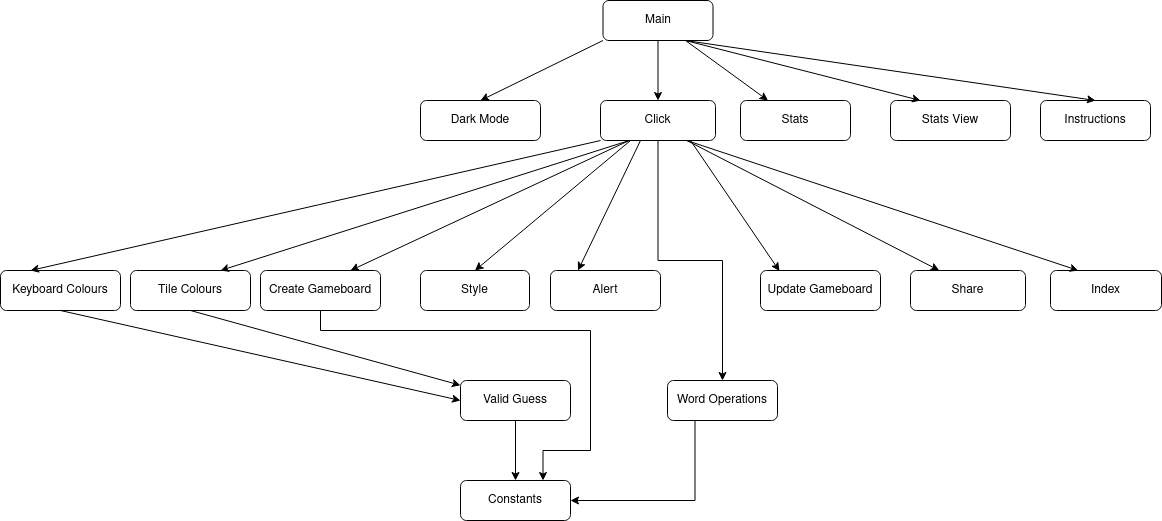
\includegraphics[width=0.7\textwidth]{useHierarchy.png}
		\caption{\textcolor{red}{Use hierarchy among modules}}
		\label{FigUH}
	\end{figure}
	
	%\section*{References}
	
	\bibliographystyle {plainnat}
	\bibliography {MG}
	
\end{document}